% --------------------------------------------------------------------------- %
% Poster for the ECCS 2011 Conference about Elementary Dynamic Networks.      %
% --------------------------------------------------------------------------- %
% Created with Brian Amberg's LaTeX Poster Template. Please refer for the     %
% attached README.md file for the details how to compile with `pdflatex`.     %
% --------------------------------------------------------------------------- %
% $LastChangedDate:: 2011-09-11 10:57:12 +0200 (V, 11 szept. 2011)          $ %
% $LastChangedRevision:: 128                                                $ %
% $LastChangedBy:: rlegendi                                                 $ %
% $Id:: poster.tex 128 2011-09-11 08:57:12Z rlegendi                        $ %
% --------------------------------------------------------------------------- %
\documentclass[a0paper,portrait]{baposter}

\usepackage{relsize}		% For \smaller
\usepackage{url}			% For \url
% \usepackage{epstopdf}	% Included EPS files automatically converted to PDF to include with pdflatex

%%% Global Settings %%%%%%%%%%%%%%%%%%%%%%%%%%%%%%%%%%%%%%%%%%%%%%%%%%%%%%%%%%%

\graphicspath{{pix/}}	% Root directory of the pictures 
% \tracingstats=2			% Enabled LaTeX logging with conditionals

%%% Color Definitions %%%%%%%%%%%%%%%%%%%%%%%%%%%%%%%%%%%%%%%%%%%%%%%%%%%%%%%%%

\definecolor{bordercol}{RGB}{40,40,40}
\definecolor{headercol1}{RGB}{186,215,230}
\definecolor{headercol2}{RGB}{80,80,80}
\definecolor{headerfontcol}{RGB}{0,0,0}
\definecolor{boxcolor}{RGB}{186,215,230}

%%%%%%%%%%%%%%%%%%%%%%%%%%%%%%%%%%%%%%%%%%%%%%%%%%%%%%%%%%%%%%%%%%%%%%%%%%%%%%%%
%%% Utility functions %%%%%%%%%%%%%%%%%%%%%%%%%%%%%%%%%%%%%%%%%%%%%%%%%%%%%%%%%%

%%% Save space in lists. Use this after the opening of the list %%%%%%%%%%%%%%%%
\newcommand{\compresslist}{
	\setlength{\itemsep}{1pt}
	\setlength{\parskip}{0pt}
	\setlength{\parsep}{0pt}
}

%%%%%%%%%%%%%%%%%%%%%%%%%%%%%%%%%%%%%%%%%%%%%%%%%%%%%%%%%%%%%%%%%%%%%%%%%%%%%%%
%%% Document Start %%%%%%%%%%%%%%%%%%%%%%%%%%%%%%%%%%%%%%%%%%%%%%%%%%%%%%%%%%%%
%%%%%%%%%%%%%%%%%%%%%%%%%%%%%%%%%%%%%%%%%%%%%%%%%%%%%%%%%%%%%%%%%%%%%%%%%%%%%%%

\begin{document}
\typeout{Poster rendering started}

%%% Setting Background Image %%%%%%%%%%%%%%%%%%%%%%%%%%%%%%%%%%%%%%%%%%%%%%%%%%
\background{
	\begin{tikzpicture}[remember picture,overlay]%
	\draw (current page.north west)+(-2em,2em) node[anchor=north west]
	{\includegraphics[height=1.1\textheight]{background}};
	\end{tikzpicture}
}

%%% General Poster Settings %%%%%%%%%%%%%%%%%%%%%%%%%%%%%%%%%%%%%%%%%%%%%%%%%%%
%%%%%% Eye Catcher, Title, Authors and University Images %%%%%%%%%%%%%%%%%%%%%%
\begin{poster}{
	grid=false,
	% Option is left on true though the eyecatcher is not used. The reason is
	% that we have a bit nicer looking title and author formatting in the headercol
	% this way
	%eyecatcher=false, 
	borderColor=bordercol,
	headerColorOne=headercol1,
	headerColorTwo=headercol2,
	headerFontColor=headerfontcol,
	% Only simple background color used, no shading, so boxColorTwo isn't necessary
	boxColorOne=boxcolor,
	headershape=roundedright,
	headerfont=\Large\sf\bf,
	textborder=rectangle,
	background=user,
	headerborder=open,
  boxshade=plain
}
%%% Eye Cacther %%%%%%%%%%%%%%%%%%%%%%%%%%%%%%%%%%%%%%%%%%%%%%%%%%%%%%%%%%%%%%%
{
	Eye Catcher, empty if option eyecatcher=false - unused
}
%%% Title %%%%%%%%%%%%%%%%%%%%%%%%%%%%%%%%%%%%%%%%%%%%%%%%%%%%%%%%%%%%%%%%%%%%%
{\sf\bf\huge
	Sleep State Prediction Using Accelerometry Data:\\
A Systematic and Computational Approach
}
%%% Authors %%%%%%%%%%%%%%%%%%%%%%%%%%%%%%%%%%%%%%%%%%%%%%%%%%%%%%%%%%%%%%%%%%%
{
	\vspace{0.6em} Juan Carlos Quintero Rubiano, Juan Felipe Wilche Gomez, Juan Nicolas Diaz Salamanca\\
	{\large jcquinteror@udistrital.edu.co, jfwilchesg@udistrital.edu.co, jndiazs@udistrital.edu.co}
}
%%% Logo %%%%%%%%%%%%%%%%%%%%%%%%%%%%%%%%%%%%%%%%%%%%%%%%%%%%%%%%%%%%%%%%%%%%%%
{
% The logos are compressed a bit into a simple box to make them smaller on the result
% (Wasn't able to find any bigger of them.)
\setlength\fboxsep{0pt}
\setlength\fboxrule{0.5pt}
	\fbox{
		\begin{minipage}{12em}
			\includegraphics[width=10em,height=10em]{my-img/logo.png}

		\end{minipage}
	}
}

\headerbox{Introduction}{name=problem,column=0,row=0}{
\large
Sleep disorders affect a significant portion of the population,
manifesting as disruptions to normal sleep patterns. Accurate
identification of sleep states is crucial for diagnosing these
disorders and evaluating treatment efficacy. Traditionally, sleep
monitoring relies on polysomnography (PSG) however due to cost and 
specialized laboratories, accelerometers is shown as a low-cost alternative
for sleep state prediction, this paper addresses the central question: How can
accelerometer data be used to accurately predict sleep state.
}

\headerbox{Input data analyzed}{name=definitions,column=0,below=problem}{
\large
\textbf{Wrist movement}: Intensity and temporal patterns of
movement, as measured by the accelerometer.\\
\textbf{Movement speed}: Changes in velocity over time, derived
from the raw acceleration data.\\
\textbf{Timestamp}: Mark the exactly time which the data was recorded,
useful to identify between data.\\
No environmental or physiological data are 
available in this analysis.
}

\headerbox{Models}{name=models,column=0,below=definitions}{
\large
\textbf{Threshold-based algorithms}: These use simple rules
based on movement intensity to distinguish sleep from
wake. For example, the Sadeh and Cole-Kripke algorithms are widely used in actigraphy-based sleep scoring \\
\textbf{Machine learning} Supervised classifiers such as random forests, support vector machines, and logistic regression are trained
on labeled data to improve classification accuracy \\
\textbf{Deep Learning}: Recurrent neural networks (RNNs), con-
volutional neural networks (CNNs), and hybrid models
are increasingly used to capture temporal dependencies
and complex patterns in accelerometry data. \\
}

\headerbox{References}{name=references,column=0,below=acknowledgments}{
\smaller													% Make the whole text smaller
\vspace{-0.4em} 										% Save some space at the beginning
\bibliographystyle{plain}							% Use plain style
\renewcommand{\section}[2]{\vskip 0.05em}		% Omit "References" title
\begin{thebibliography}{1}							% Simple bibliography with widest label of 1
\itemsep=-0.01em										% Save space between the separation
\setlength{\baselineskip}{0.4em}					% Save space with longer lines
\bibitem{prevWork1} Laszlo Gulyas, Richard Legendi: \emph{Effects of Sample Duration on Network Statistics in Elementary Models of Dynamic Networks}, International Conference on Computational Science, Singapore (2011) 
\bibitem{prevWork2} Laszlo Gulyas, Susan Khor, Richard Legendi and George Kampis \emph{Cumulative Properties of Elementary Dynamic Networks}, The International Sunbelt Social Network Conference XXXI (2011)
\bibitem{gulya-kampis1} Gulyas, Laszlo et al.: \emph{Betweenness Centrality Dynamics in Networks of Changing Density}. Presented at the 19th International Symposium on Mathematical Theory of Networks and Systems (MTNS 2010)
\end{thebibliography}
}

\headerbox{Conclusion}{name=acknowledgements,column=0,below=models, above=bottom}{
					
\vspace{-0.1em}
\large% Save some space at the beginning
Accelerometers measures present a low-cost and non-invasive alternative with consistent accurate reported sensitivity values of 91-93 percent for actigraphy compared to PSG and advanced machine learning techniques, particularly sequence models like LSTMs, achieve the best accuracy in binary sleep/wake classification. 
However, several limitations over distinguish between all sleep stages
(e.g., REM vs. non-REM) with high accuracy, and it may misclassified periods of quiet wakefulness as sleep. Also the absence of environmental and physiological data constrains the precision of accelerometry based model.
} 

\headerbox{Sleep state systematic approach}{name=density,span=2,column=1,row=0}{
Sleep stages are divided by biophysiological changes during sleep on the parameters: \textbf{EEG (Brain activity)}, \textbf{EOG (Eye movements)}, \textbf{EMG (Muscle tone)}, \textbf{ECG (Heart rate)}. According to American Academy of Sleep Medicine (AASM) guidelines, these measurements allow classification of sleep into five distinct stages (Wake, N1, N2, N3, and REM):
\vspace{1em}
\centering
\includegraphics[width=10cm, height=7cm]{my-img/sleepStages.png}
\\
\vspace{1em}
\textbf{SLEEP STAGES MEASUREMENTS SYSTEM DIAGRAM}
\\
\vspace{1em}
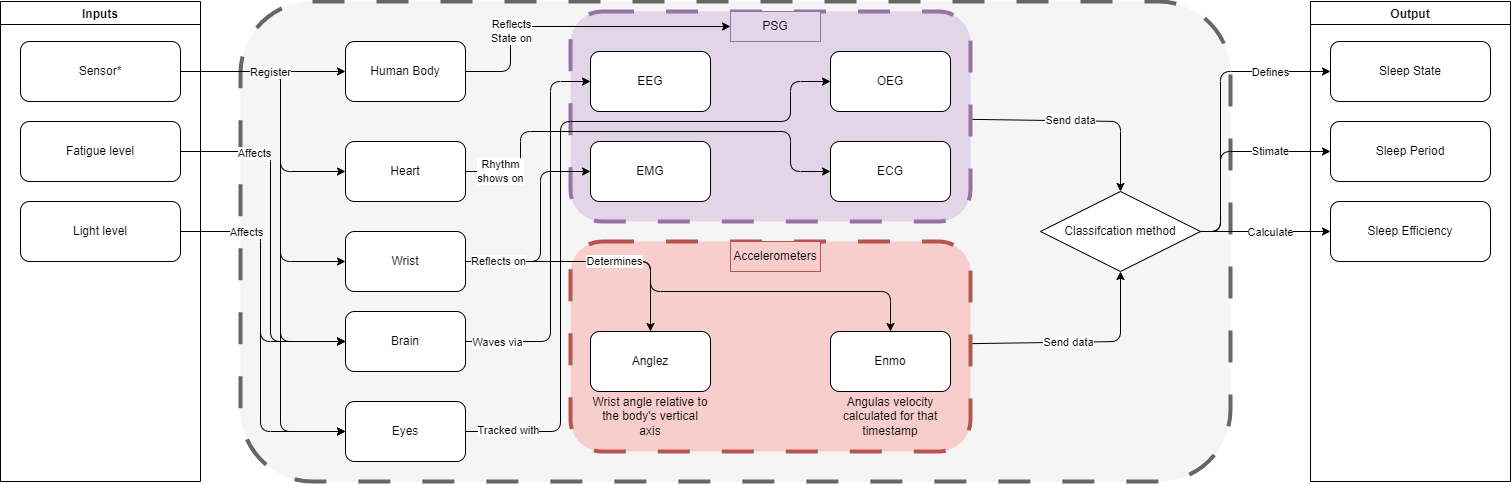
\includegraphics[width=15cm, height=7cm]{my-img/sleep_system_diagram.png}
\vspace{1em}
}
\vspace{1em}
\headerbox{Sleep state computational approach}
{name=degreeDistribution,span=2,column=1,below=density,above=bottom}{
The computational model processes raw accelerometry data to extract features such as: \\
•Activity counts: The sum of absolute acceleration
changes over fixed time epochs (typically 30-second
or 1-minute windows), providing a measure of overall
movement intensity.\\
• Movement variability: Standard deviation and entropy
of accelerometer signals, which can distinguish between
different sleep states.\\ 
• Frequency-domain features: Spectral power in different 
frequency bands, extracted using Fourier transforms, capturing 
rhythmic movements characteristic of different
sleep states.\\
• Temporal patterns: Sequences of activity/inactivity, du-
rations of inactive periods, and transitions between active
and inactive states.\\
These features are input to classify each time segment as sleep or wake period.
\vspace{1em}
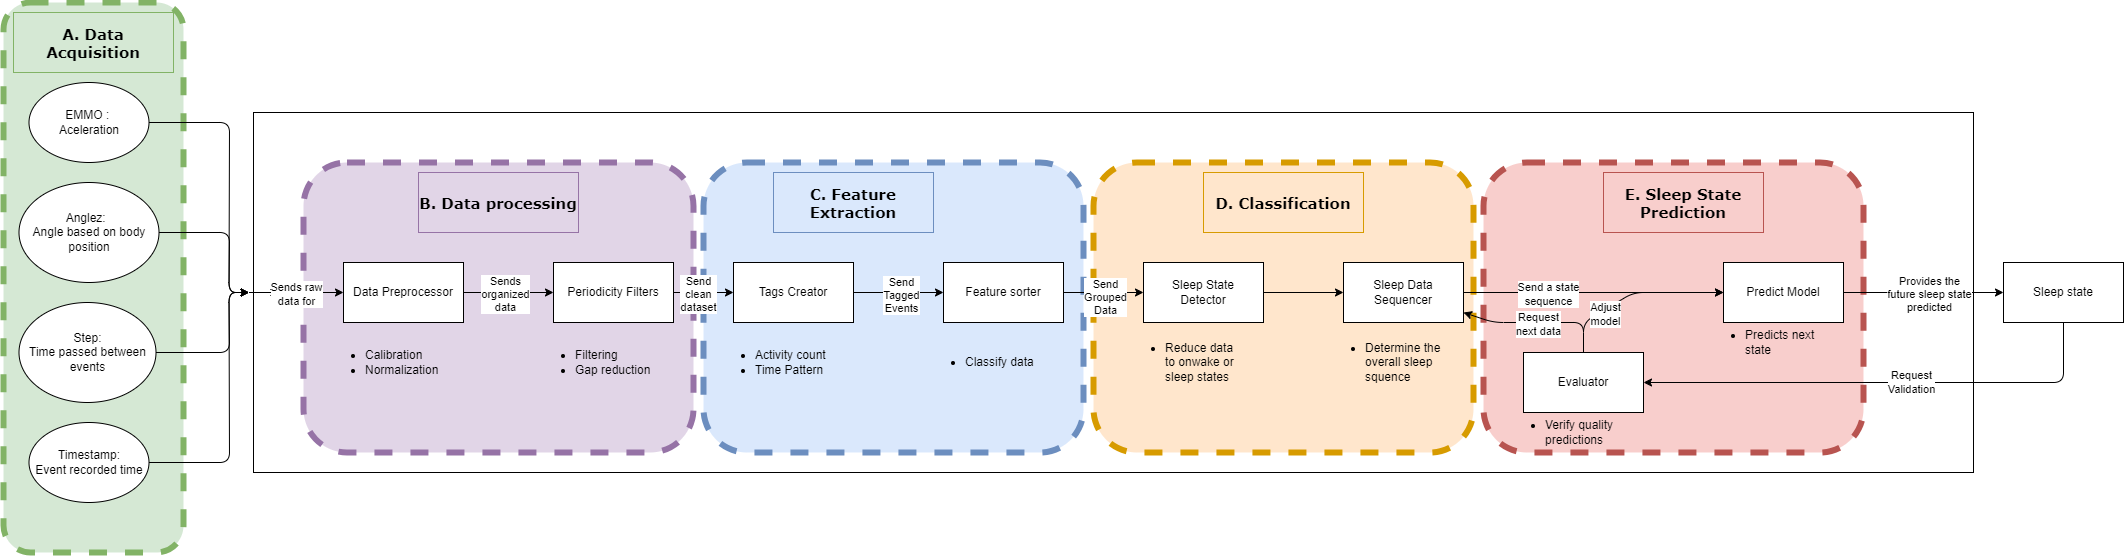
\includegraphics[width=15cm, height=6cm]{conceptual_model.png}
}
\end{poster}
\end{document}